\chapter{Discussions}
This final chapter is divided in X sections. First, an account of direct observations that may inform the focus of future research on the test. Second the analysis of early testing sessions to see how reliable initial settings of the test can be. Third, we discuss the limitations of the test and the question of interpretability of the scores. Fourth, we elaborate on the direction that future research on the topic would look like. Finally, we present a conclusion gathering all the contributions of the dissertation as well as an informed answer to the research question.

\section{Direct Observations}
The information presented here are insights from the author on others' attitude and results when passing the test. They are not supported by data, but only direct observations, and as such they may be subject to biases. However they bring light to blind spots that could not have been foreseen when designing the test.

\subsection{Age and the Relationship to Risk}
When looking at people taking the Breton test for the first time, older people seemed to score better than young people. I recall particularly two young people who were scholarized bilingual schools until age 18, and kept using the language to some extent later, whereas at least one elderly person had no formal education in Breton, and never read books in the language, learning the language through causual social interactions only. It is well possible that older people just have a lot of vocabulary, but the surprise was more how low the score of the young people was. Knowing that these young adults were capable of having fluent conversations in Breton, they are expected to know the most frequent words, yet they both scored below 500. To this day, we see two explaination for this trend. Either the vocabulary acquired by a passive exposition to the language in school may be suboptimal. Either the behaviour of younger people when facing unknown word is different. Older people taking the test took a lot of time to pounder each answer. Younger people took the test quickly, and seemed less risk averse, maybe ready to accept meaning where there is none, or maybe unwilling to recognise their ignorance and limitations. Because of how harsh the score was downgraded when recognising non-words, this unforeseen variation in people's relationship to risk might cause variations in the Breton vocabulary test, regardless of absolute fluency and vocabulary level. It is the reason why the pseudo-words ratings were initialized within the 0–2000 range for the other languages.

Unfortunately there is no more to it than these direct comments. But this observation on the relationship to risk seem consistent with research in social science \parencite{wang_does_2023}. Accounting for this behavioural independant variable in the scoring system was envisaged, like by modeling the tendency to recognize distractors and somehow have the final score maping more to the absolute level in vocabulary recognition skills, if this is even possible while accounting for cheating strategies. This idea was put aside however, for two reasons. For one, the test are intended for self assessment, to measure the progression of individuals through time, not to compare level between students. Secondly, as the test is intended for repeated usage, it is expected that test takers will eventually adapt their behaviour to ``make peace with their ignorance'', be it in order to maximise their results.

\subsection{Worth of the Test as a Learning Tool}
As an advanced beginer in Ukrainian, the author is regularly exposed to the language in an immersion setting. The analysis functionality of the test has proven to be a remarkably useful learning tool. A tool that complement the oral exposition to the language with tailored written feedback, fostering generalisation skills. In the lower range of ratings there are comparatively few items to select from. This means that the test takers are likely to run into these few items in any testing session. In this range, idea that the unrecognised real words in a test session are the next most useful words to learn is really strong. The initial aim behind building a test was to build a technological brick that would help optimize later teaching programs. But it turned out that being able to accuratly answer the question ``Where to start with now''? is already a monumental part in any teaching process. The simple LLM-based feedback, although imperfect seems like the unexpectedly most useful aspect of the test so far. But of course, it relies on everything else that has been discussed so far.

\subsection{Ceiling effects}
\begin{figure}
    \centering
    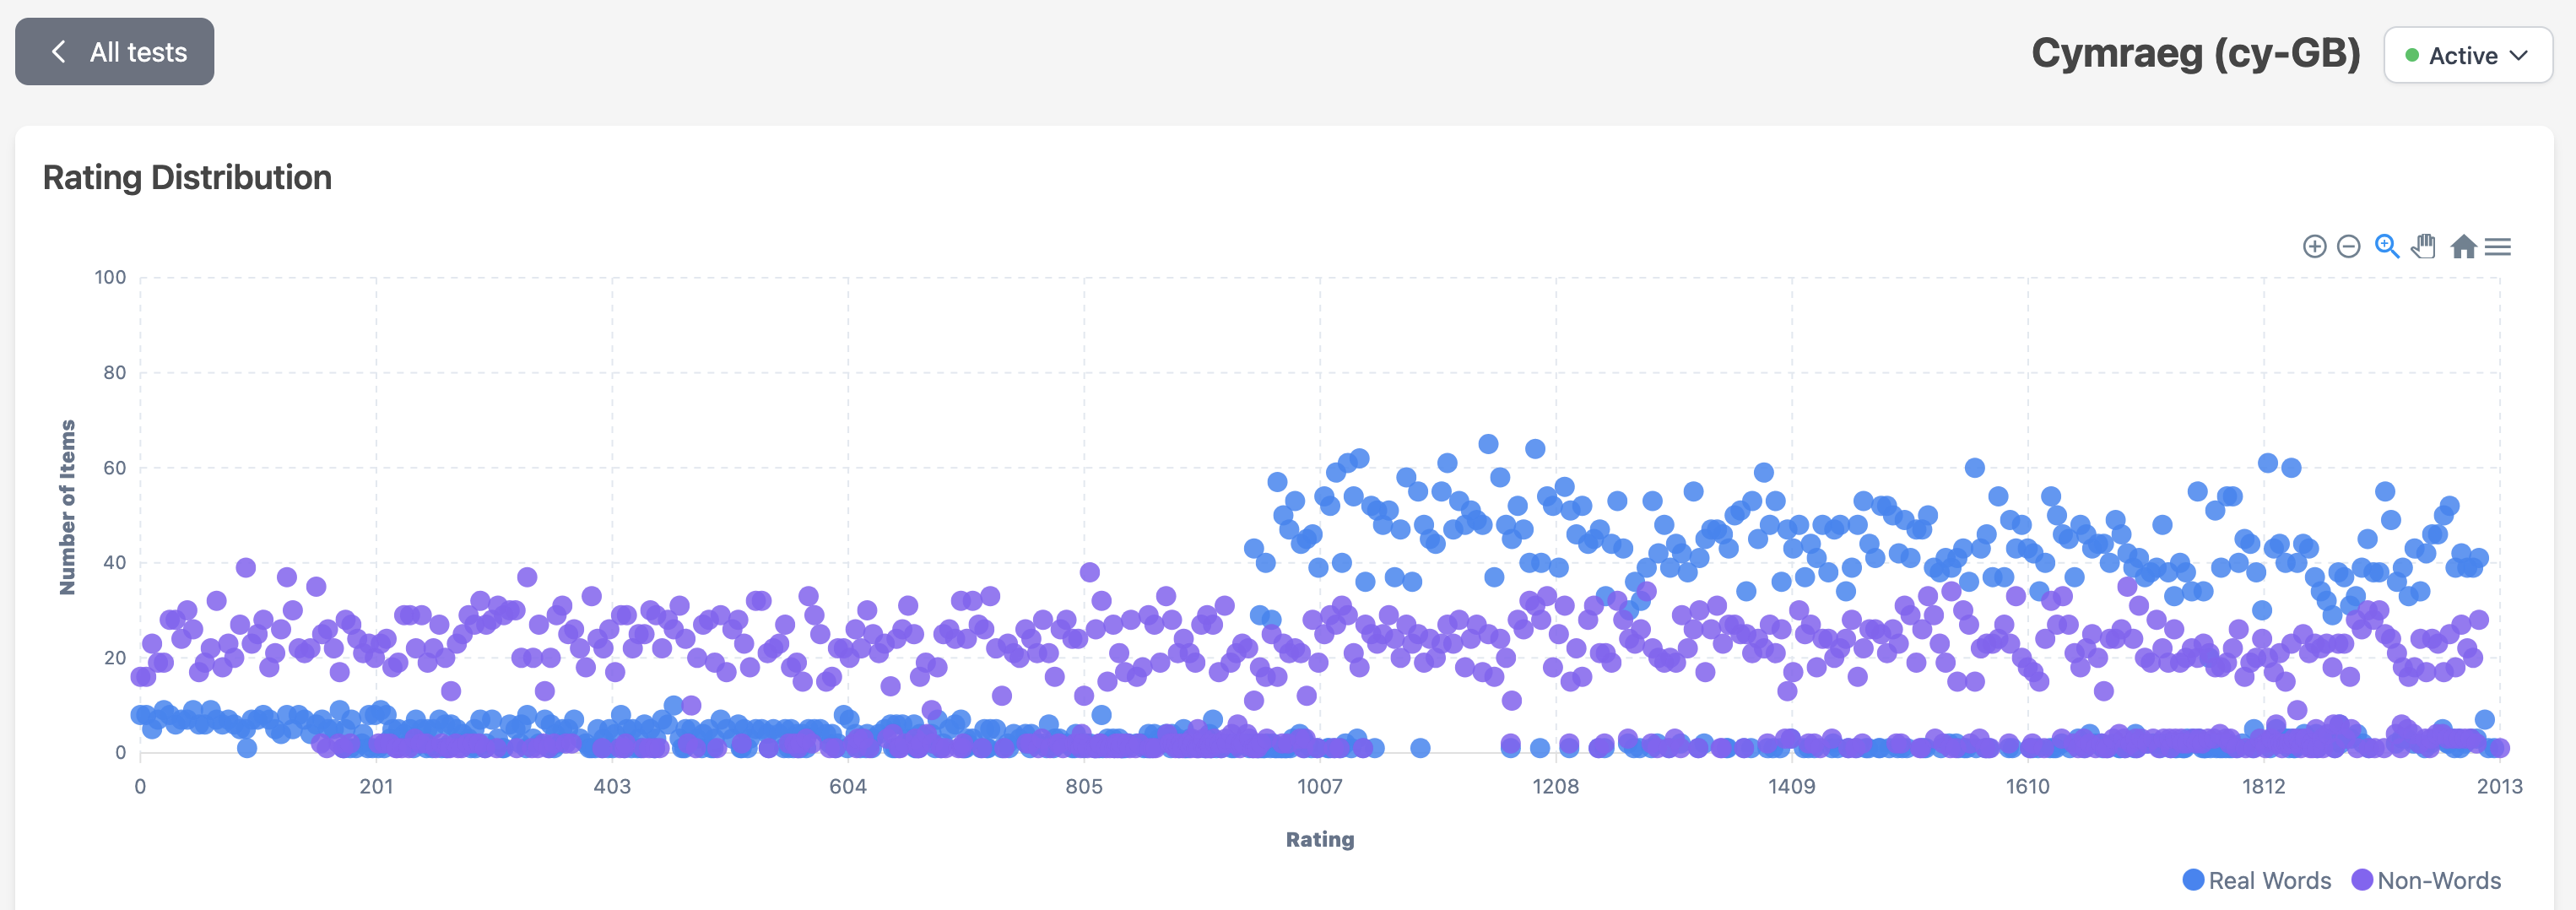
\includegraphics[width=0.8\linewidth]{figures/cy-distribution.png}
    \caption{Distribution of the items in the Welsh tests}
    \medskip
    \small
    We can see that the early test takers had answered a lot of items in the high-900 range and around 1800 level, with a gap in the 1000–1300 range. This looks like a strong indicator of a ceiling effect in the higher range of the test and a ``bottleneck'' effect in the transition between the items rated ramdomly and those rated by frequency rank.
\end{figure}\label{fig:cy-distribution}

All these observations on potential ceiling are based upon preliminary observation and not supported by data. Yet, these may be of interrest to orient future research on this specific phenomenon. 

The Welsh test is the one containing the fewest items so far, only 10722 real words, with rating spreading between 0 and 2000. Some of the few people who have taken it reported a rating around the 2000. This seem to be a strong indicator that a test that does not contain enough items will exhibit a ceiling effect around the highest rated items' rating. However, even when the pool the available items seem much larger, like in Ukrainian, the same problem seemed to remain. The explaination for this is simple. The initial assupmtion was that the tests would behave between a Elo rating system and a proportion-based system, with the items in the 1000–2000 range being randomly rated. But when a test taker knows more than half of the items in the 1000–1300 range, they ultimately know most of the items in the 1700-2000 range. In this initial setting, there is no reason for there rating to stabilize somewhere in the middle. This means that such a large random spread of less frequent real words is unjustified. At most the words not included in a frequency list should be initially spread in the 1000–1400 range. Of course, a ceiling effect would be observed for the first few test sessions, but this is unavoidable. On the other hand, the calibration process would happen much faster. If a relatively easy word has to end up somewhere in the 950–1000 range, it will reach this position faster from an initial 1300 or 1400 rating, than from a 1000 or 2000 rating. The same goes in reverse. The reason for proposing the 400 range span, is the interpretation of the Elo ratings. 400 difference in rating means a 90\% chance of success. So test takers recognising most the randomly distributed items in this range are initially granted a rating that means they have around 90\% chances to recognise the easiest items from this range.
Because the ratings are capped to zero, there are little chances that a ceiling effect would appear in the bottom of the scale. Only a few recognised real-words are needed to reach a positive final score.

The problem of the transition from the 0–1000 range (randomly rated within ranges defined on frequency lists) to the 1000+ range (randomly rated within one large range) is tighly linked to the problem mentioned earlier. The easiest items from the upper band must make their way down as fast as possible. To ensure a smoother transition in this critical junction, we propose that the two ranges be spaced from one another. The gap would be filled by the harder items from the frequency lists and the easiest randomly rated items. A gap of 100 points, would not slow down the progression of the test takers ratings.

\section{Test Sessions Analysis}
\subsection{Brier Score}
The Brier score is the most straight-forward way to measure the accuracy in a series of a statistical prediction. We'll use it to analyze our sessions. Because we are only interrested by the knowledge of the test takers, and not their relationship to non-sense words, we shall only consider the real words in these results. The Brier score is defined by the following equation.

\begin{equation}
    BS=\frac{1}{N}\sum^{N}_{t=1} (f_t - o_t)^2
\end{equation}\label{eq:brier-score}

Where $(f_t - o_t)^2$ is the squared difference between the predicted outcome (of a real word) and the actual outcome. However, as the test did only store the final user rating (x axis), the value of $o_t$ is constant each test session. This can help us inspect how the pseudo words affect the final results. In figure \ref{fig:brier}, we see that many of the lower ratings also correspond to the worst brier scores. This means that many unlikely outcomes happened in these sessions. Most likely, these unlikely events are recognition of many words rated above the final score. This would be an indication of many pseudo-words being recognised, which, as we discussed already, may be either the fruit of a cheating strategy, or a higher tolerance to risk.  Unfortunately, it does not seem that much more observation can be taken from so few results.

\begin{figure}
    \centering
    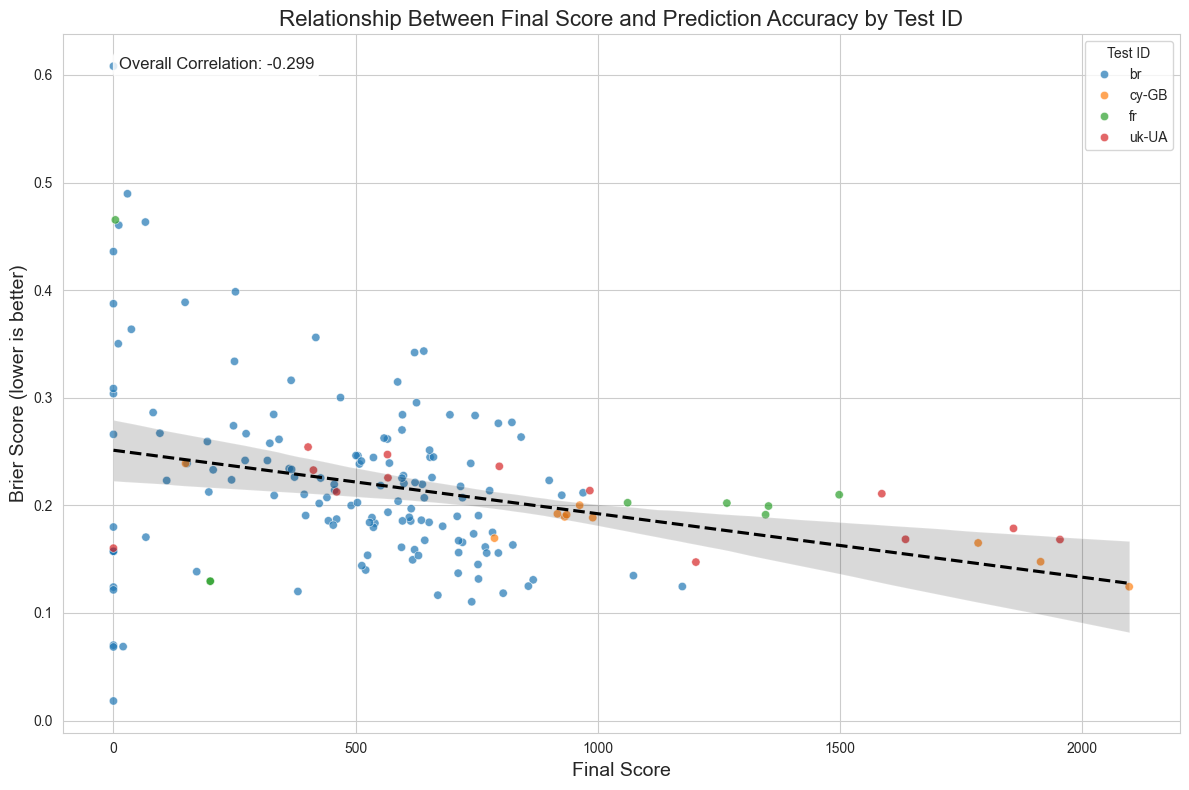
\includegraphics[width=0.8\linewidth]{figures/brier_score.png}
    \caption{Brier scores by rating, the colors represent different langauges}
    \medskip
    \small
    
\end{figure}\label{fig:brier}

Now that this preliminary analasys is made, it seems that it would have been wiser to also collect the current rating of the test taker, and not only the final one. This modification in the test result may allow deeper analysis.Wwith enough sessions stored, we could for example highlight bottlenecks or ceiling effect by making a mean difference for each rating range of a test. If some critical ranges show big deviations from the norm, it would show a ceiling effect. But this would require a larger adoption of the test.

\subsection{Measuring Adaptivity}
As mentioned in the previous chapter, we can use the last real-word recognition to test adaptivity. For the sake of consistency, we only consider the results of the Breton test, which has the most results. 142 test sessions were gathered in the results. The number of last real words recognised in the last round of a test is 73, which makes 51.4\%. If we were trying to prove the hypothesis of faulty calibration of the system, we would need a p-value bellow 0.05. However, the current results yeld a p-value of 0.801339022, which is really high, and thus does not invalidate the corresponding null hypothesis that the chances of recognising the last real word are highly uncertain.
This result is highly encouraging in many ways. Firstly, only three categories of real words were used to pre-calibrate the items in the test. The benefits of using the modulo clusters to create an hybrid system between proportion of correct answers and a classic logistic scale is thus conforted. Second, the level of pressision claimed is really high. The pression is defined by the uncertainty function \ref{uncertainty-function}. It is variable, because dependant on the the number of real words seen in the session, number which depends on the length of length of the session, which dependents on the rating. Unfortunately, the final value of the uncertainty function was not stored. It is at most ±52, if no word is recognised, and go down as the rating goes up.
As the early results on testing the adaptivity of the test were encouraging, we propose to extend the analysis to specific ranges. The result are given in the following table.

\begin{table}[h]
\centering
\begin{tabular}{|c|c|c|c|c|c|}
\hline
\textbf{ranges} & \textbf{sessions} & \textbf{recognised last word} & \textbf{observed mean} & \textbf{expected} & \textbf{p-value} \\
\hline
(0, 100] & 10 & 6 & 0.600000 & 0.5 & 0.753906 \\
(100, 200] & 7 & 1 & 0.142857 & 0.5 & 0.125000 \\
(200, 300] & 7 & 2 & 0.285714 & 0.5 & 0.453125 \\
(300, 400] & 12 & 6 & 0.500000 & 0.5 & 1.000000 \\
(400, 500] & 14 & 6 & 0.428571 & 0.5 & 0.790527 \\
(500, 600] & 29 & 16 & 0.551724 & 0.5 & 0.711071 \\
(600, 700] & 22 & 12 & 0.545455 & 0.5 & 0.831812 \\
(700, 800] & 22 & 13 & 0.590909 & 0.5 & 0.523467 \\
(800, 900] & 7 & 6 & 0.857143 & 0.5 & 0.125000 \\
(900, 1000] & 8 & 3 & 0.375000 & 0.5 & 0.726562 \\
(1000, 1100] & 2 & 1 & 0.500000 & 0.5 & 1.000000 \\
(1100, 1200] & 1 & 1 & 1.000000 & 0.5 & 1.000000 \\
(1200, 1300] & 2 & 0 & 0.000000 & 0.5 & 0.500000 \\
(1300, 1400] & 2 & 2 & 1.000000 & 0.5 & 0.500000 \\
(1400, 1500] & 1 & 0 & 0.000000 & 0.5 & 1.000000 \\
(1500, 1600] & 1 & 0 & 0.000000 & 0.5 & 1.000000 \\
(1600, 1700] & 1 & 0 & 0.000000 & 0.5 & 1.000000 \\
(1700, 1800] & 1 & 1 & 1.000000 & 0.5 & 1.000000 \\
(1800, 1900] & 1 & 0 & 0.000000 & 0.5 & 1.000000 \\
\hline
\end{tabular}
\caption{Recognition Statistics by Score Ranges}
\label{tab:recognition_stats}
\end{table}

As can be seen, the low number of session for each range does not allow to unvalidate the null hypothesis, that the last real word chance of being recognised are random. However, the null hypothesis can not be validated neither, we can only state that the result are so far consistant with it. Note that this method seem to be able to show early signs of potential ceiling effects. The transition from below to above 900 seems to show potential ceiling effects. The range 800–900 has a higher mean than 85\%, when the 900–1000 range drops to 37\%. Once again, the sample size is to small to confirm the presence of a significant ceiling effect. But this method of analysis could show such issues if a test is used at a larger scale. On the other hand, a wider adoption of the test would a better calibration, and thus improve the results. All the code for these results can be found on github\footnote{See this link \url{https://github.com/Oktogazh/analeksis/blob/master/analeskis.ipynb}}.

\section{Limitations and Interpretation of the Scores}
An easy misinterpretation to make about the test score would be to consider all the words below a final score as mastered by the test takers and those rated above the final score as unrecognisable by them. This is not exactly what the reasults imply. The final score is supposed to represent the level at which a student recognise only 50\% of the words, without necessarly understanding their meaning. An item rated 677 points less than the final score has 99\% chances of being rightfully recognised. Conversely, an item rated 677 points more than a final score would be recognised 1\% of the time. As there are more items in the higher ranges, if the final score is in the lower ranges, this 1\% is ``bigger'' than the 1\% of few items in lower ranges. In simples terms, this means that, indeed, almost all words in the lower ranges below a given rating are expected to be well known, (including with a stronger understanding of their meanings). But many words in the higher range could still be recognised.

This test looks for a breaking point in the student knowledge, rather that showing exactly all the words that they know. Comparing again with the CEFR paradigm, which is based on a ``can-do'' approach \parencite{europe_common_2020}, this paradigm looks for the ``can't-do''. In practice it will work the same for a majority of cases, because of the normative nature of the Elo system update mechanism. However, an potential limitation is to be highlighted here.

People are not to be expected to learn languages the same ways. When using a same language as children, partners, students, scholars, tourists, professionals or missionaries, people may need to use master divergent lexical fields. To which extend the vocabulary of these different learners overlaps is an open question. Whether or not this divergence in usage contradicts the statistical interpretation presented above is another question. Eventually, it may become relevant to build clone vocabulary tests in order to target different demographies within the same language. Cloning the test may be the best way to ensure a proper deduction of the ``can-do'' from the ``can't-do'.

\section{Future Research}
We see three different directions of research going forward. The first is about the study of eventual ceiling effects in the tests, and the speed at which the calibration of a test can be considered completed. This aspect is essential to measure the dynamics of language acquisition. The second is about pedagogy, as the test can already be used at least for measuring ``milestone'' levels in vocabulary aquisition. This could be used to experiment on different pedagogical approaches, \textbf{including in diglossic settings}. Finally, the test could be pushed further, including in non-WEIRD environment to study language use divergence and evaluate the need for domain-specific scales.

The two first directions could be researched in parallel with relatively little efforts, by focusing around adult classes of regional languages like Welsh. This would in effect turn the lack of resources and the limited reach of LRLs in a research advantage. The third one would necessitate more resources and most likely international cohordination, with different social groups involved and would likely focus on HRLs.

In the broader field of AIED, the modulo clustering technique appear to be a promising way to build future MCQ tests, whose items would have been mass generated by LLMs. This method could be used to both calibrate their relative difficulty and measure the students level and progress in other fields than L2 acquisition. Other potential research could focus on simulations, to find out what are the optimum parameters (modulo base, spread of the initial items etc...) to build such tests.

\section{Conclusion}
Overall, this vocabulary test design showed that the focus on higher-resource languages in the study of language acquisition is not a fatality. Many challenges have been overcome in this dissertation, although we may end up with more new questions than answers. Luckily, these questions are asked along with clear methods for analysis and a refutable hypothesis. Coming back to the original question, all the element collected in this work cannot disprove the idea that quick language tests can be created for low resource languages. The only remaining questions are, how reliable and precise can they get with an imperfect calibration.

Additionally, it seems to be a good measure to seek to integrate future research on the topic more closely in the usage context of these languages. The initial motivation of this work was the optimization of low resource language teaching. But in this context, can the word optimisation be understood in the sense of getting more by doing less? Based on the elements gathered in this dissertation, it seems that human skills always grow to fit their usage needs. In this regard, it may well be that the thing that needs the most to be optimised is the time spent using these languages. That is, getting more by doing more, and admitting there is no reason think a technological shortcut exists for a problem that is primarly social. Hopefully, a quick vocabulary test score may become a way to give subtance and increase awareness to the value of this cumulated usage. 
